%%%%%%%%%%%%%%%%%%%%%%%%%%%%%%%%%%%%%%%%%%%%%%%%%%%%%%%%%%%%%%%%
%%                          CHAPTER 2                         %%
%%%%%%%%%%%%%%%%%%%%%%%%%%%%%%%%%%%%%%%%%%%%%%%%%%%%%%%%%%%%%%%%
\chapter{The synchroniser compiler}
  \section{Mathematical Model}
Synchroniser $S = (\Phi, \; \Pi)$, where
  \begin{itemize}
  \item[] $\Phi = (A, \; S, \; T)$ -- nondeterministic state machine:
    \begin{itemize}
    \item[] $A \subseteq C \times P$ -- the alphabet of events, $C$ -- set of synchroniser input channels, $P$ -- set of predicates on channel messages. An event $(c, \; p) \in A$ represents the reception of a message on channel $c$ that satisfies predicate $p$,
    \item[] $S \supseteq \{s_{0}\}$ -- set of abstract states, $s_{0}$ -- start state,
    \item[] $T \: : \: A \times S \to S$ -- transition matrix.
    \end{itemize}
  \item[] $\Pi \: : \: S \times \Omega \to V$ -- path functional that defines the synchroniser output:
    \begin{itemize}
    \item[] $\Omega$ -- the set of output channels,
    \item[] $V$ -- the set of message values \cite{astrakahn}.
    \end{itemize}
  \end{itemize}

In a state $s_{k}$ the functional is based on the retrospective sequence of transitions from the most recent visit to the start state $s_{0}$ to $s_{k}$:
  \begin{itemize}
  \item[] $(s_{0}, c_{0}), \: (s_{1}, c_{1}),... \: (s_{k}, c_{k})$, where
    \begin{itemize}
      \item[] $s_{0}$ -- start state,
      \item[] $c_{i} \in C$, $0 \le i \le k$ -- the channel that caused the transition from the state $s_{i}$.
    \end{itemize}
  \end{itemize}

Let $\mu_{i}$ be the message received in the transition from the state $s_{i}$. Then
  \begin{itemize}
  \item[] $\Pi \; (s_{k}, \omega_{m}) = \psi_{\sqcap} \; \{\mu_{i} \: | \: \rho_{ki}^{m} \; (s_{i}), \: 0 \le i \le k\}$, where
    \begin{itemize}
      \item[] $\rho_{ki}^{m}$ -- selection predicate that defines $\Pi$,
      \item[] $\psi_{\sqcap}$ -- the operator that coerces the messages in the operand set to their joint greatest subtype.
    \end{itemize}
  \end{itemize}

From the above, the synchroniser is fully defined by two functions:
  \begin{enumerate}
  \item The transition matrix $T$

The state machine can have a regular structure whereby many transitions can be defined at once by a formula with some limited range integer variables. For example, a machine with 8 states could have a transition matrix defined thus: $S_{k \; mod \; 8} \to S_{k+1 \; mod \; 8}$.

In order to be able to use regular structures, \ak\ allows synchronisers to declare \emph{state} variables.

\textbf{Example: the counter synchroniser}  Counter emits every $n$-th message received in its input channel to the output channel. The transition diagram for the counter synchroniser for $n = 3$ is given in Figure \ref{fig:counter}.a.

Mathematical model $S_{counter_{3}} = (\Phi, \; \Pi)$, where
  \begin{itemize}
  \item[] $\Phi = (A, \; S, \; T)$,
    \begin{itemize}
    \item[] $C = (a)$, $P = (true)$, $A = C \times P = ((a, \; true))$,
    \item[] $S = (s_{0}, \; s_{1}, \; s_{2})$, $s_{0}$ -- start state,
    \item[] $T$:
      \begin{tabular}{c|c|c|c}
      $A$ \textbackslash $S$ & $s_{0}$ & $s_{1}$ & $s_{2}$\\
      \hline
      $(a, \; true)$ & $s_{1}$ & $s_{2}$ & $s_{0}$\\
      \end{tabular}
    \end{itemize}
  \item[] $\Pi \: : \: S \times \Omega \to V$,
    \begin{itemize}
    \item[] $\Omega = (c)$,
    \item[] $V = (a)$
    \end{itemize}
  \end{itemize}

An output message is emitted when a transition happens from the state $s_{2}$. This state is reached in a single path:
  \begin{itemize}
  \item[]
$W_{0} = ((s_{0}, \; a), \: (s_{1}, \; a), \: (s_{2}, \; a))$
% fixed rho{1i}^{c} to rho{2i}^{c}
$\Pi \; (s_{2}, c) = \psi_{\sqcap} \; \{\mu_{0} = a \: | \: \rho_{20}^{c} \; (s_{0}) = 0, \mu_{1} = a \: | \: \rho_{21}^{c} \; (s_{1}) = 0, \mu_{2} = a \: | \: \rho_{22}^{c} \; (s_{2}) = 1\}$, $k = 1$, $i = 0,1,2$ 
  \end{itemize}

The state machine behind the counter has a regular structure, and for this synchroniser all its transitions may be defined with a single formula: $S_{k \; mod \; 3} \to S_{k+1 \; mod \; 3}$. Considering this, the transition matrix $T$ would be:
  \begin{tabular}{c|c}
  $A$ \textbackslash $S$ & $S_{k \; mod \; 3}$\\
  \hline
  $(a, \; true)$ & $S_{k+1 \; mod \; 3}$
  \end{tabular}

Some possible transition diagrams of the counter synchroniser are given in Figure \ref{fig:counter}. The diagram \ref{fig:counter}.a represents the unrolled regular structure of the synchroniser. However, this representation is inconvenient when $n \gg 1$. The transition diagram \ref{fig:counter}.a can be folded using state variables. Two possible variants are shown in figures \ref{fig:counter}.b and \ref{fig:counter}.c. The state variable $c$ acts as an induction variable in a while loop with the exit condition $c \ge 3$.

  \begin{figure}[here]
  \centering
  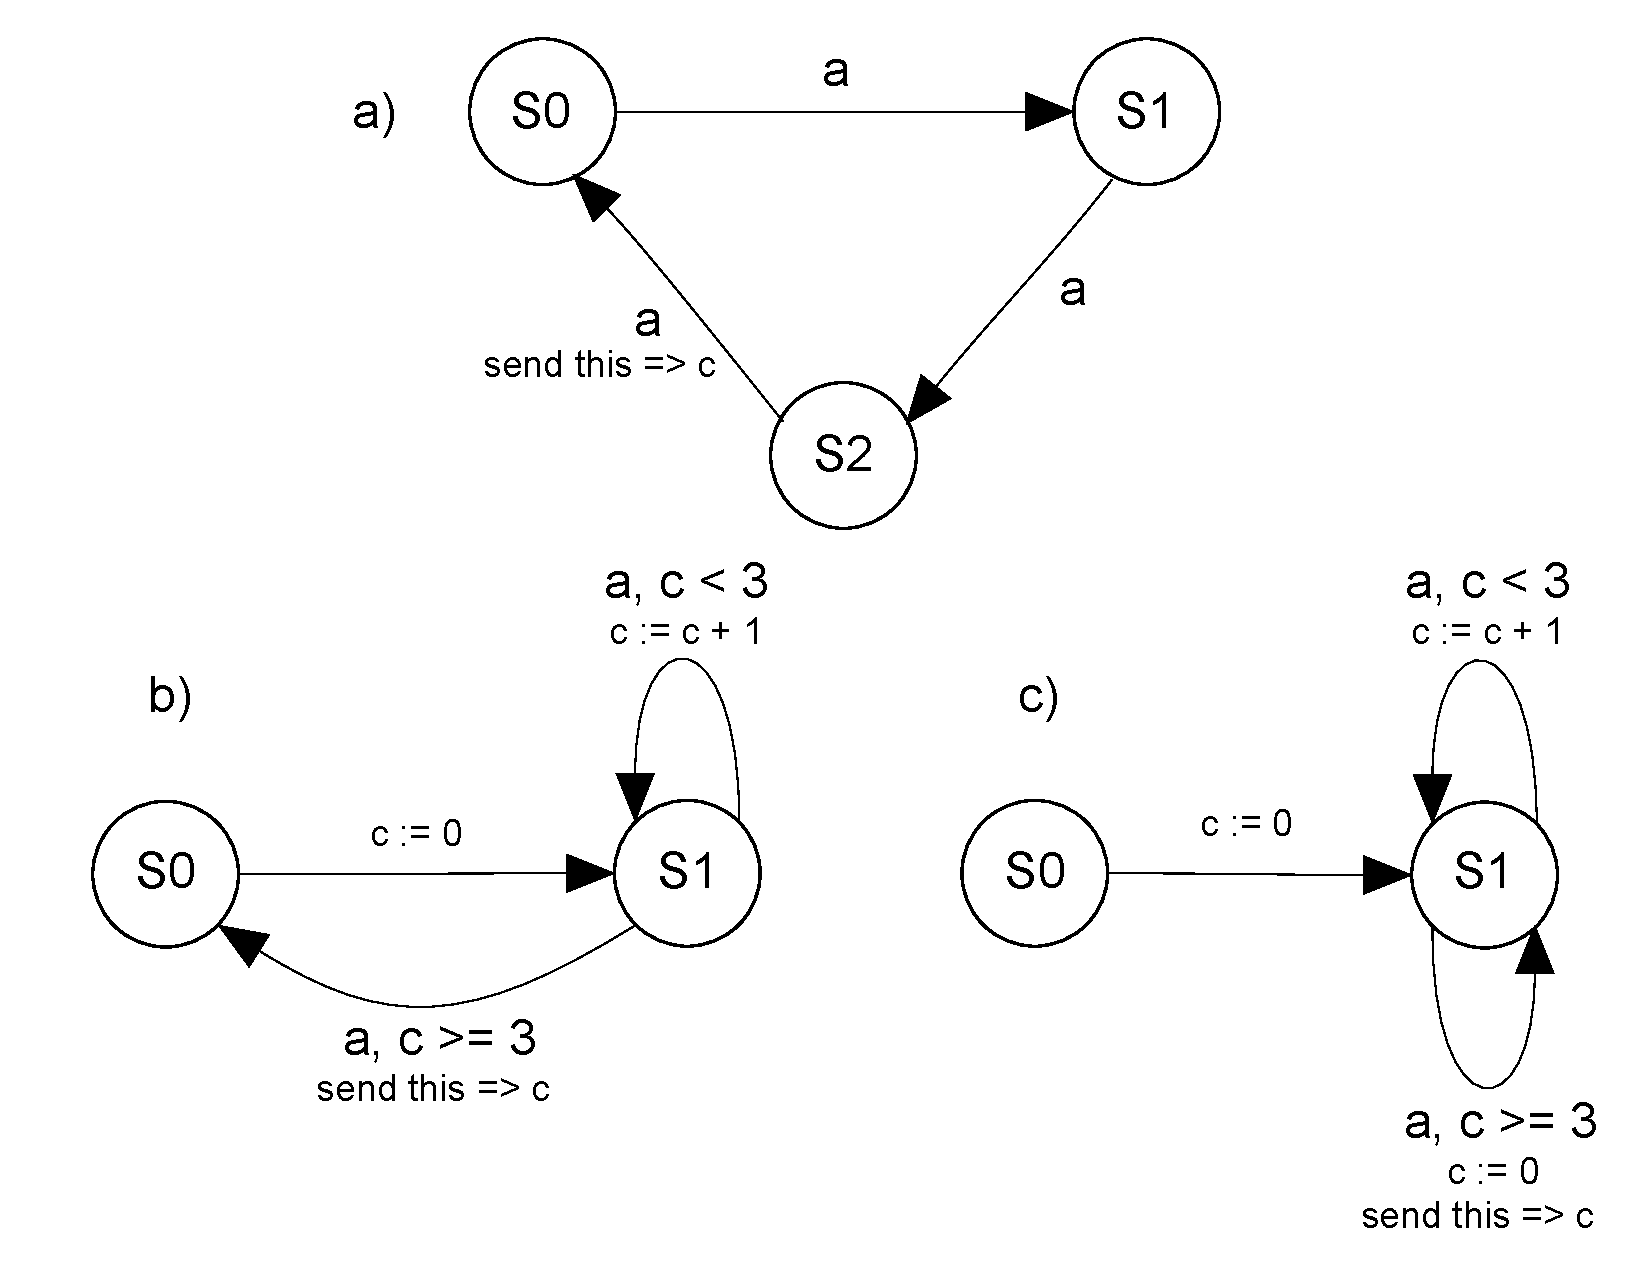
\includegraphics[scale=0.4]{figs/counter.pdf}
  \caption{The transition diagrams of the counter synchroniser.}
  \label{fig:counter}
  \end{figure}


  \item The selection predicate $\rho$

In a given state $k$ for each output channel $\omega_{m}$ we note all $i$ on which $\rho_{ki}^{m}$ is true. Those message values must be stored in a previous state and recalled in state $k$. It is expected that the boolean vector $\omega_{i} = \rho_{ki}^{m}$ has only very few true elements.

Consequently the storage mechanism that \ak\ provides for synchronisers is in the form of individual \emph{store} variables. The type of a store variable is determined when a variable is assigned.

\textbf{Example: the binary zip synchroniser}  Zip2 receives messages on its input channels and sends their concatenation to the output channel. In the resulting concatenation there's exactly one message from each input channel and those messages are ordered as they received.

The zip2 transition diagram is given in Figure \ref{fig:zip2}. The message received in the current transition is referred by a keyword \emph{this}. $ma$ and $mb$ are the store variables associated with the input channels $a$ and $b$ respectively. The statement \emph{send} indicates a sending of a message to an output channel.

  \begin{figure}[here]
  \centering
  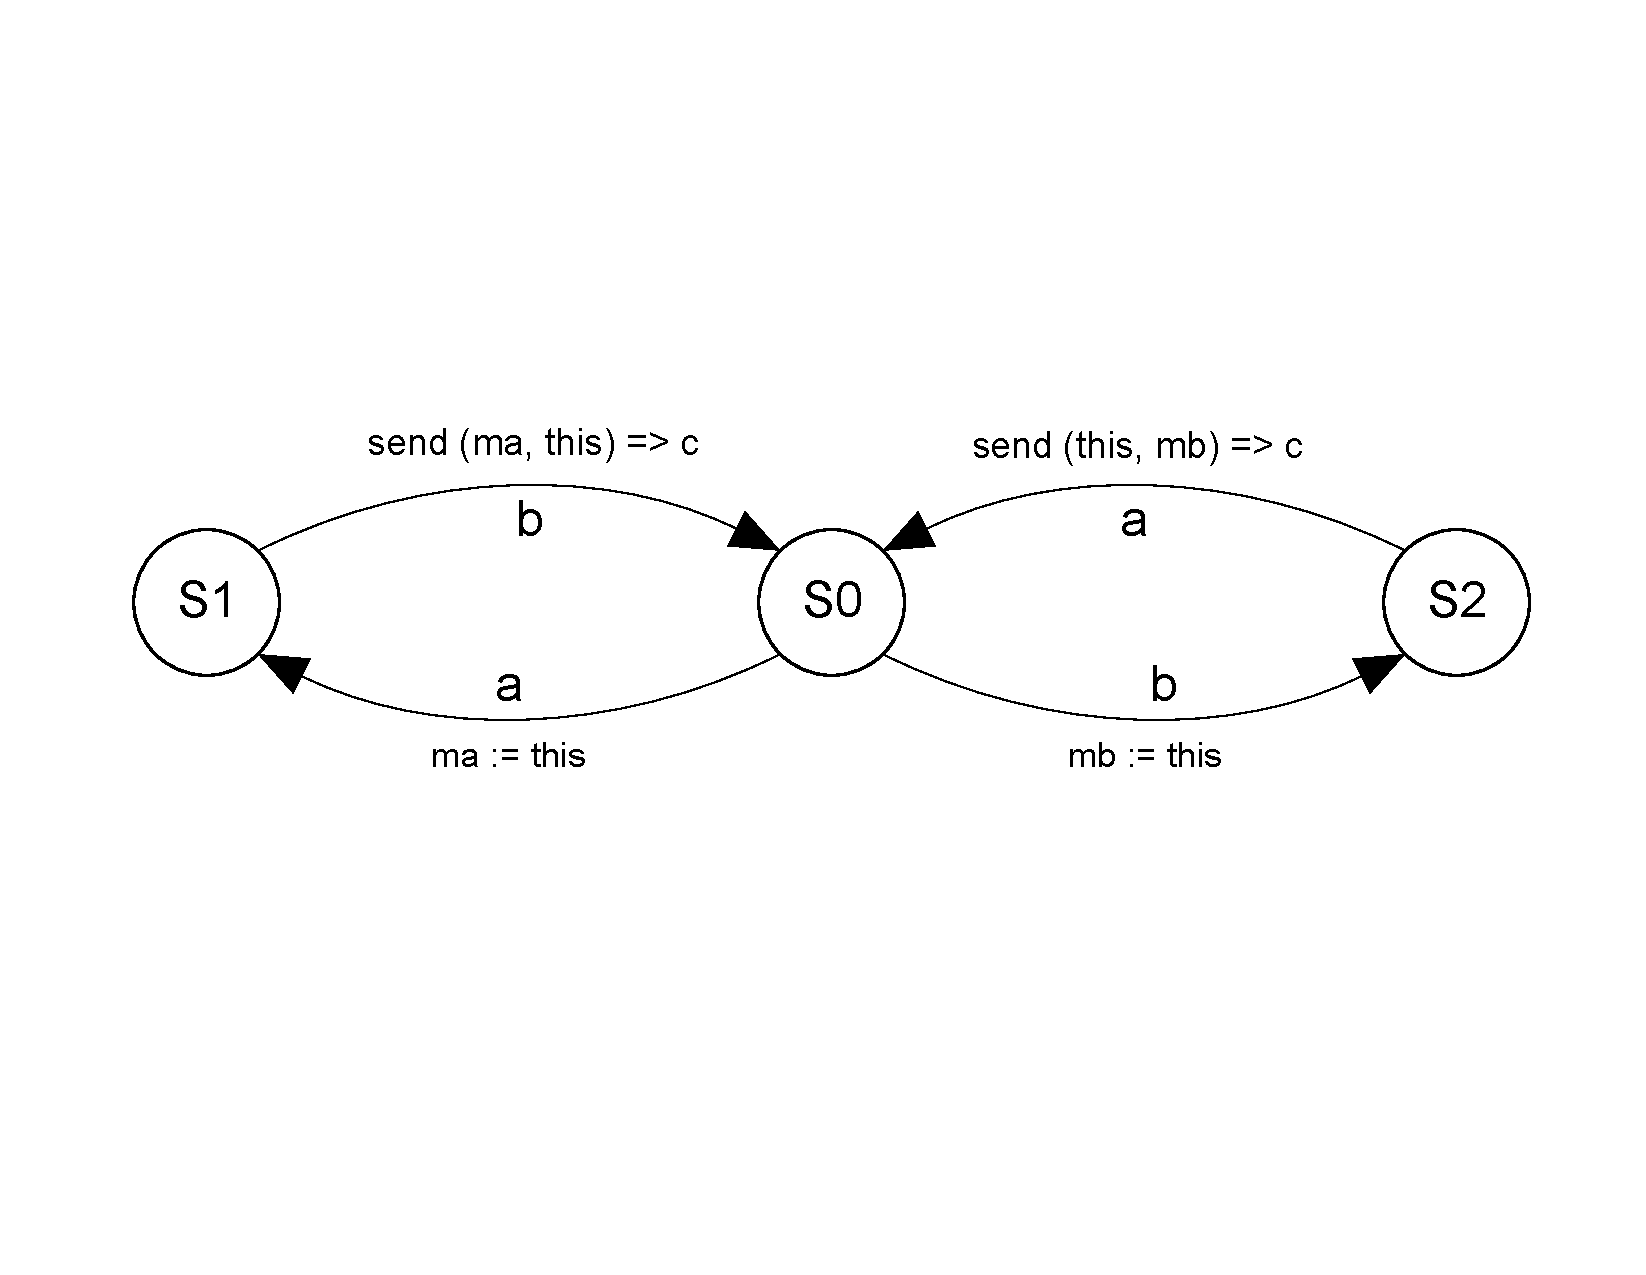
\includegraphics[scale=0.4]{figs/zip2.pdf}
  \caption{The transition diagram of the zip2 synchroniser.}
  \label{fig:zip2}
  \end{figure}

Mathematical model $S_{zip2} = (\Phi, \; \Pi)$, where
  \begin{itemize}
  \item[] $\Phi = (A, \; S, \; T)$,
    \begin{itemize}
    \item[] $C = (a, \; b)$, $P = (true)$, $A = C \times P = ((a, \; true), \: (b, \; true))$,
    \item[] $S = (s_{0}, s_{1}, s_{2})$, $s_{0}$ -- start state,
    \item[] $T$:
      \begin{tabular}{c|c|c|c}
      $A$ \textbackslash $S$ & $s_{0}$ & $s_{1}$ & $s_{2}$\\
      \hline
      $(a, \; true)$ & $s_{1}$ & $s_{1}$ & $s_{0}$\\
      \hline
      $(b, \; true)$ & $s_{2}$ & $s_{0}$ & $s_{2}$\\
      \end{tabular}
    \end{itemize}
  \item[] $\Pi \: : \: S \times \Omega \to V$,
    \begin{itemize}
    \item[] $\Omega = (c)$,
    \item[] $V = ((a, \; b), \: (b, \; a))$
    \end{itemize}
  \end{itemize}

An output message is emitted when a transition happens either from the state $s_{1}$ or the state $s_{2}$. These states are reached in two paths:
  \begin{itemize}
  \item[]
$W_{0} = ((s_{0}, \; a), \: (s_{1}, \; b))$

$\Pi \; (s_{1}, c) = \psi_{\sqcap} \; \{\mu_{0} = a \: | \: \rho_{10}^{c} \; (s_{0}) = 1, \mu_{1} = b \: | \: \rho_{11}^{c} \; (s_{1}) = 1\}$, $k = 1$, $i = 0,1$
  \item[]
$W_{1} = ((s_{0}, \; b), \: (s_{2}, \; a))$

$\Pi \; (s_{2}, c) = \psi_{\sqcap} \; \{\mu_{0} = b \: | \: \rho_{20}^{c} \; (s_{0}) = 1, \mu_{2} = a \: | \: \rho_{22}^{c} \; (s_{2}) = 1\}$, $k = 2$, $i = 0,2$ 
  \end{itemize}
  \end{enumerate}


\section{Synchroniser code}
%% TODO fix 'channel connected to the port x' to channel x
%% Insert a footer that explains that 'channel x' is short for 'channel connected to the port x'
An \ak\ synchroniser is a finite state machine, therefore the basic building blocks of a synchroniser program are states and transitions. A state of a synchroniser is fully defined by the corresponding state of the finite state machine and the values of the state variables. A transition is the act of moving to another state which is initiated by a triggering event. A triggering event for the synchroniser transition is an arrival of a message to the associated channel. The message may be required to have a specific structure. In addition, a transition may be guarded by special conditions on the values of the state variables. If the conditions are satisfied the transition fires, otherwise it is cancelled.

Once a transition is known to fire, optional actions may be performed before the underlying state machine makes the move. These actions include changing the state and store variable values and sending messages to the output channels. In order to change the state and store variables, the synchroniser language provides state and store expressions over them.

This section gives an overview of the \ak\ synchroniser programming language. The formal grammar of the \ak\ synchroniser is provided in Appendix \ref{sync_syntax}.

  \subsection{Program structure}
A synchroniser program consists of a header followed by the synchroniser's body wrapped in braces. The begining of a synchroniser program is indicated by the keyword $synch$.

The header of a synchroniser program contains the synchroniser's name and the channel signature. The name is an ASCII string that follows the C convention.

The body of the synchroniser lists the state and store variables declarations and the states of the underlying finite state machine. Each state is defined by a list of transitions. Each transition lists its triggering condition which includes an optional guarding state expression, an optional list of actions, and, finally, the destination state.

%  \subsection{Macros}
%%%
%%% We removed macros from the language. The compiler must invoke a preprocessor to expand them.
%%%
%The synchroniser language provides macros to avoid having to trivially alter synchroniser programs. Macros are specified in brackets between the synchroniser's name and its channel signature. An example of a configurable synchroniser can be found in \cite{astrakahn}.

  \subsection{Channel signature}
The channel signature defines the input channels and the output channels of the synchroniser and their bracketing depths. The synchroniser header (Fig. \ref{min_sync_head}) declares the synchroniser $min$ with two input channels that are connected to the ports $a$, $b$ and two output channels that are connected to the ports $c$, $d$. If the bracketing depths of the channels are not specified, they are assumed to be 0. Thus, the bracketing depth of the channel $a$ is 0.

The input channel depth $-1$ indicates that the input channel is ignored in the synchroniser program. The output channel with the depth $-1$ must not have data sent to them.

\begin{figure}[h!]
\begin{lstlisting}[frame=single]
synch min (a, b:p | c:2, d:p+1)
\end{lstlisting}
\caption{The synchroniser header}
\label{min_sync_head}
\end{figure}

%% TODO remove read-only state variables

The \ak\ synchroniser allows to declare constant and configurable integer depths for the input and output channels. In addition, the depth of the output channel can be specified with an integer shift to the configurable input channel depth.

The input channels are required to have the bracketing depths specified in the signature. Thus, the channel connected to the port $a$ of the $min$ synchroniser must have zero bracketing depth. The channel connected to the port $b$ has a configurable bracketing depth $p$. Actual values of configurable bracketing depths of input channels are determined by the \ak\ compiler. %Once defined in the signature, configurable bracketing depths may be used in state expressions. They are interpreted as read-only state variables.

The output channels of a synchroniser are guaranteed to have the bracketing depths specified in the channel signature. Thus, the synchroniser $min$ must send messages to the output channel connected to the port $c$ at the depth 2 and optionally at the depths $0$, $1$. The output channel connected to the port $d$ must have the bracketing depth $p+1$ that is the depth of the input channel connected to the port $b$ shifted by $1$.


%% TODO Move all the type details to the implementation details
%% TODO The width of int type is declared explicitly to reduce the number of potential states of automata.
  \subsection{Variable declaration}
%% Add about state and store variables initialisation.
%% state int(8) a, b=1, c=8; // assignes a=0 b=1 c=9
%% enum (a,b,c) foo, bar=a;  // assignes foo=0 bar=a
The beginning of state variables declaration is indicated by the keyword $state$. A state variable may be either a signed integer of the constant width or a C-style enumeration. State and store variables names are user-defined indentifiers. A user-defined identifier is an ASCII string that follows the C convention.

%% TODO Should move width determining to the implementation detail
Line 1 in Fig. \ref{sync_statevar} declares state variables $a$, $b$, $c$ of width 4. Thus, all three variables are declared to have integer values in the range $[-8; 7]$. Generally, a state variable of width $n$ has integer values in the range $[-2^{n-1}; 2^{n-1}-1]$.

The state variable $foo$ that is declared in the line 2 in Fig. \ref{sync_statevar} can only be assigned the values $d$, $e$ and $f$ specified in the enumeration. The enumeration values are defined as constants if type $int$. If the values are not specified explicitly, they are assigned consequtive positive integers starting with 0. The width of the $int$ type is $\lceil \log_{2}{n} \rceil + 1$, where $n$ is the number of values in the enumeration. Thus, the variable $foo$ has integer values $d=0$, $e=1$ and $f=2$ of the width $\lceil \log_{2}{3} \rceil + 1 = 3$. If the values are specified explicitly, the width is determined as $\lceil \log_{2}{(m+1)} \rceil + 1$, where $m$ is the biggest value in the enumeration. For the variable $bar$ declared in line 3 of Fig. \ref{sync_statevar} $m=4$ and the width is $\lceil \log_{2}{(5)} \rceil + 1 = 4$.

Integer state variables and enum values can be mixed freely in state expressions. Enum values are interpreted as read-only integer state variables. % constant integers!

\begin{figure}[h!]
\lstset{numbers=left, numberstyle=\small, stepnumber=1, numbersep=8pt}
\begin{lstlisting}[frame=single]
state int(4) a, b, c;
state enum(d, e, f) foo;
state enum(x = 1, y = 2, z = 4) bar;
store msg_a, msg_b;
\end{lstlisting}
\caption{State and store variables declaration}
\label{sync_statevar}
\end{figure}

Store variables declaration begins with a keyword $store$. Line 4 in Fig. \ref{sync_statevar} declares state variables $msg\_a$ and $msg\_b$. Store variables do not need explicit type specification; their types are determined on the first assignment to the variable.

All the state and store variables are global to all the synchroniser states.


  \subsection{States and transitions}
States and transitions of the synchroniser define which channels are read and in what order. Fig. \ref{zip_struc} presents the code of the binary zip synchroniser's state machine. Line 1 declares the start state of the synchroniser. The $on$ clause indicates the beginning of the transitions list. In the start state the zip2 synchroniser acceptes messages from both input channels $a$ and $b$. State and store expressions associated with the transition and the destination state are specified in the braces.

\begin{figure}[h!]
\lstset{numbers=left, numberstyle=\small, stepnumber=1, numbersep=8pt}
\begin{lstlisting}[frame=single]
start {
  on:
    a { goto s1;    }
    b { goto s2;    }
}
s1 {
  on:
    b { goto start; }
}
s2 {
  on:
    a { goto start; }
}
\end{lstlisting}
\caption{State machine of the zip2 synchroniser}
\label{zip_struc}
\end{figure}

When the zip2 synchroniser is in the start state and it receives a message from the channels connected to the port $a$, the underlying state machine makes a transition to the state $s1$. In this state the synchroniser can only receive messages from channel connected to the port $b$ since there's no transition triggered by channel connected to the port $a$ and defined in this state. When the message on channel connected to the port $b$ is received, the state machine makes a transition to the start state. Lines 10-13 define similar behaviour in state $s2$.

%% Change 'scopes'. 'Blocks' probably
The synchroniser language supports top-down prioritised transition scopes. They are indicated with the $elseon$ keyword. A synchroniser in state $foo$ in Fig. \ref{sync_scope} acceptes messages from channels connected to the ports $a$, $b$, $c$ and $d$. When no destination state is specified for a transition, a synchroniser makes the transition to the current state. If all channels are ready at the same time in state $foo$, the synchroniser processes messages from either channel $a$ or $b$ first. When all messages from channels connected to the ports $a$ and $b$ are processed the synchroniser receives messages from channels connected to the port $c$. If there're no messages in channels $a$, $b$ and $c$ the synchroniser receives messages from the channel connected to the port $d$.

\begin{figure}[h!]
\lstset{numbers=left, numberstyle=\small, stepnumber=1, numbersep=8pt}
\begin{lstlisting}[frame=single]
foo {
  on:
    a { }
    b { }
  elseon:
    c { }
  elseon:
    d { }
}
\end{lstlisting}
\caption{Prioritised transition scopes}
\label{sync_scope}
\end{figure}


  \subsection{State expressions}
State expression is a combination of integer constants, state variables and operators, which computes and produces an integer value. The interpretation of a state expression follows C rules of precedence and association. State expressions can be assigned to state variables. In assumption that the output channel is infinite a synthetic example in Fig. \ref{sync_state_exp} counts the number of messages received from channel connected to the port $a$ between the arrivals of messages in channel connected to the port $b$. Line 1 declares the 8-bit integer $count$ and initialises it with 0. When a message from channel connected to the port $a$ is received the value of $count$ increases by 1 (line 5).

\begin{figure}[h!]
\lstset{numbers=left, numberstyle=\small, stepnumber=1, numbersep=8pt}
\begin{lstlisting}[frame=single]
state int(8) count = 0;
foo {
  on:
    a {
      set count = [count + 1];
    }
  elseon:
    b {
      set n = [count], count = [0];
      send count:[n] => c;
    }
}
\end{lstlisting}
\caption{Use of state variables and expressions}
\label{sync_state_exp}
\end{figure}

When a message from channel connected to the port $b$ is received the value of $count$ is stored in the temporary variable $n$, set to 0 and then $n$ is sent to the output channel.

The variable $n$ does not have to be declared and is considered alias for the integer expression. Temporary variables are available until the state machine of a synchroniser makes the next move.


  \subsection{Triggering of a transition}
The channel name on its own stands for the availability predicate for the corresponding channel, i.e. the condition that a message of any kind is available. Whether a transition takes place depends on the channel status and optionally the content of the messages.

When a message is received on a channel, it can be matched with a pattern in order to extract parameters needed to select a specific transition. Line 3 of Fig. \ref{sync_trans} checks if a message received from the input channel connected to the port $a$ contains label $x$. If it does, the contents of $x$ are stored in a temporary variable $x$. The tail of the message, i.e. everything but the part labeled $x$, is stored in a temporary variable $t$. Both $x$ and $t$ are read-only and available until the state machine makes a move.

\begin{figure}[h!]
\lstset{numbers=left, numberstyle=\small, stepnumber=1, numbersep=8pt}
\begin{lstlisting}[frame=single]
foo {
  on:
    a.(x || t)  { }
    a.?v        { }
    a.?v(x, y)  { }
    a.@[k]      { }
}
\end{lstlisting}
\caption{Message content extraction}
\label{sync_trans}
\end{figure}

To support message formats where several variants of a message are possible, a qualifier \begin{bf}?\end{bf}$\alpha$ is available as an input condition. It qualifies input messages as belonging to $\alpha$ variant. Line 4 of Fig. \ref{sync_trans} checks if a message received from channel connected to the port $a$ belongs to the variant $v$. Line 5 checks that a message that belongs to the variant $v$ contains only two records labeled $x$ and $y$. 

A channel carries a stream that consists of messages and possibly segmentation marks. In line 6 in Fig. \ref{sync_trans} a message is checked if it is a segmentation mark of the depth $k$. The depth of a segmentation mark can be a state expression.

Several different channels can be tested in any given state, however, once the readiness of a channel was established, the synchroniser is committed. Hence the set of conditions applied to the message on any input channel must be exhaustive. In Fig. \ref{sync_trans} it is not, because there no pattern for messages that do not contain label $x$, do not belong to variant $v$ and are not a segmentation mark of depth $k$ at the same time. In this case the final clause $a$\begin{bf}.else;\end{bf} is assumed. This clause discards the input message and transitions the synchroniser back to its current state.

A transition can be guarded by a state expression. In this case the transition fires only if the guarding expression evaluates to true. The synchroniser in Fig. \ref{sync_g_state_exp} sends every 256-th message to the output channel. Line 1 declares the 8-bit state variable $i$ that is initialised with 0. It is incremented every time a message from channel connected to the port $a$ is received, except when it reaches 255, in which case it is reset 0 and the received message is sent down the channel $c$. 

Values that are matched from the message can be used in guarding state expressions.
\begin{figure}[h!]
\lstset{numbers=left, numberstyle=\small, stepnumber=1, numbersep=8pt}
\begin{lstlisting}[frame=single]
state int(8) i;
start {
  on:
    a & [i < 255] {
      set i = [i + 1];
    }
    a & [i = 255] {
      set i = [0];
      send this => c;
    }
}
\end{lstlisting}
\caption{Use of guarding state expressions}
\label{sync_g_state_exp}
\end{figure}


  \subsection{Store expressions and sending messages}
%% TODO Probably fix it after writing about CAL terms.
Store expression is a mechanism to combine data. Data are typed in \ak\. Types are CAL terms. Store expression concatenates data in the user-defined order and therefore results in the data of a valid CAL type. The result of the store expression can be either stored in a store variable or sent down the output channel.

The example in Fig. \ref{sync_send} demonstrates the use of store expressions and the $send$ clause. In the start state the synchroniser receives messages from channel connected to the port $a$ that has label $n$ in it. In line 5 the value under label $n$ is incremented and stored in the store variable $ma$ under label $n$ together with the tail $t$. The syntactic sugar for defining a record is supported. The operator $'$ applied to the variable $x$ creates the record $'x': value(x)$.

%% TODO Provide a more convincing example for 'id and this
\begin{figure}[h!]
\lstset{numbers=left, numberstyle=\small, stepnumber=1, numbersep=8pt}
\begin{lstlisting}[frame=single]
store ma;
start {
  on:
    a.(n || t) {
      set ma = (n:[n+1] || t);
      goto s1;
    }
}
s1 {
  on:
    b {
      send ma || this => c;
      goto start;
    }
}
\end{lstlisting}
\caption{Use of store expressions and the $send$ clause}
\label{sync_send}
\end{figure}

A message received on a channel is referred to by the keyword $this$ within the active transition. In state $s1$ the synchroniser receives messages from channel connected to the port $b$. When a message is received, it is concatenated with the store variable $ma$ (line 12) and sent to the output channel connected to the port $c$.


%% TODO Probably move to implementation details
  \subsection{Keywords, reserved words and punctuation}
The keywords, the reserved words and the punctuation used in the \ak\ synchroniser sytax are shown in Fig. \ref{sync_kw}.
\begin{figure}[h!]
\centering
\begin{tabular}{|c|p{0.7\textwidth}|}
\hline
Keywords & synch, store, state, int, enum, start, on, elseon, else, do, send, goto\\
\hline
Reserved words & nil, this\\
\hline
Punctuation & braces, brackets, parantheses, the comma, the dot, the semicolon, the plus sign, the minus sign, the ampersand, the at sign, the question mark, the bar-bar sign, the equality sign, the arrow\\
\hline
\end{tabular}
\caption{\ak\ synchroniser keywords, reserved words and punctiation}
\label{sync_kw}
\end{figure}
 

\section{Execution order of synchroniser\label{execod}}
\begin{itemize}
\item Fairness policy
\item on-elseon execution order, dead $elseon$ code with <chan>$.else$
\item Non-deterministic $goto$
\item Algorithm of the execution of synchronisers
\end{itemize}


\section{The implementation of the compiler}
The implementation of the compiler is written in Python (TODO: cite a cookbook), with code generation to an intermediate representation that is used by the \ak\ runtime system.

\subsection{Lexical analysis}
  \paragraph{Lexical analyser} PLY
  \paragraph{Preprocessor}
%%%
%%% We removed macros from the language. The compiler must invoke a preprocessor to expand them.
%%%
%The synchroniser language provides macros to avoid having to trivially alter synchroniser programs. Macros are specified in brackets between the synchroniser's name and its channel signature. An example of a configurable synchroniser can be found in \cite{astrakahn}.
Preprocessor performs (a C-like) macro expansion. There's no preprocessor directives in the synchroniser language (like \#define in C). Preprocessor commands are passed to it as a part of the compiler invocation command (a special flag like -Dday=night in C).


\subsection{Syntax analysis}
  \paragraph{Syntax alanyser} PLY. Syntax-directed translation. A translation scheme embeds program fragments called semantic actions in production bodies (TODO Dragon book, p.107)

  \paragraph{Abstract syntax tree} The result of syntax analysis is a representation of the source program called intermediate code. We use abstract syntax tree in the implementation.

TODO: structure of the AST.
AST generator by Eli with the reference.

  \paragraph{Symbol table}
Symbol tables are data structures used by compilers to hold information about identifiers in a program's source code. The information is collected incrementally by the analysis phases of a compiler. Entries in the symbol table contain identifier's type, scope level, location and any other relevant information.

The role of a symbol table is to pass information from declarations to uses. A semantic action puts information about identifier $x$ into the symbol table, when the declaration of $x$ is analysed. Subsequenlty, a semantic action associated with a production that involves an identifier gets information about the identifier from the symbol table.

The scope of a declaration is the portion of a program to which the declaration applies. (TODO scope straucture of a sync program). State and store variables are visible for all transitions, therefore they belong to the global scope. State expression aliases and variables that are pattern matched belong to the local scope of a transition.

Symbol tables typically need to support multiple declarations of the same identifier within a program. We shall implement scope by setting up a separate symbol table for each scope (transition) and chaining them. The approach to the implementation of a symbol table is taken from (TODO ref Dragon book, p.89). Chaining of symbol tables results in a tree structure (probably we can simplity it somehow, because we do not really need a tree of scopes).

(TODO: probably a short description of the approach is needed. Class with fields hashtable and a link to the previous scope object, and methods 'create new', 'put', 'get' which searches the chain of tables.)

The symbol table contains types and (possibly) locations. Builing of a symbol table Dragon book p.90.

  \paragraph{Syntax-driven type inference?}
Special language constructs simplify type inference (probably it's not a good word here).
A state expression is specified in brackets. Everything in state expression is integer.
If an assignment is being parsed and no brackets were specified in assignment expression, then it is a store expression.

  \paragraph{Static checking}
Static checks are consistency checks that are done during compilation. Not only do they assure that a program can be compiled successfully, but they also catch programming errors early. Static checking includes:
\begin{itemize}
\item Syntactic checking. Constraints such as an identifier is declared at most once in a scope (TODO: more)

Reserved words $nil$ and $this$ can't be identifiers

\item Type checking. The type rules of a language assure that an operator or function is applied to the right number and type of operands.

If an identifier was met and it is already in the current scope of symbol table, it must have the same type (int or data) as before.
\end{itemize}

\subsection{Semantic analysis}
  \paragraph{Semantic analyser}
Architecture of the analyser. Pattern visitor?

  \paragraph{Checks}
\begin{enumerate}
\item Channel signature. If the output channel depth is in the form of depth expression $p+integer$, then $p$ should be the depth of one of the input channels. $p$ is not allowed anywhere in state expressions.
  \begin{itemize}
  \item (a:p | b:p+1) - allowed
  \item (a:p | b:0) - allowed
  \item (a:p | b:r) - allowed
  \item (a:p | b:r+1) - NOT allowed
  \end{itemize}
The special depth $-1$ indicated that the channel is not used. Therefore, if it is an input channel, all the transitions reading from it can be removed. If it is an output channel, and the transition that sends to this channel is valid, then an error must occur.

Visitor for ports that returns their depths which are IDs.
For the input and output channels sets that are returned by the visitor are equal.
Do we really need visitor for it?

\item State variables.
State variables are in global scope.

int(n) a, b, c; n denotes only the value range of a state variable. It decreases the number of possible states of a synchroniser. $a$, $b$ and $c$ must always be within range $[0; 2^{n}-1]$ (int is unsigned). At low level state variables are machine- and target language- dependent integers.

The translation scheme in Fig. \ref{std} presents state variable types and their ranges.

(Table: grammar rule - type/width, p.375 Dragon book).
\begin{figure}[h!]
\centering
\begin{tabular}{|c|c|}
\hline
Type & Values\\
\hline
int(n) & $[0; 2^{n}-1] \cap \mathbb{Z}$\\
\hline
enum($a_1$, $a_2$, $\dots$ $a_n$) & $[0; n-1] \cap \mathbb{Z}$\\
\hline
enum($a_1=N_1$, $a_2=N_2$, $\dots$ $a_n=N_n$) & $N_1$, $N_2$, $\dots$ $N_n$\\
\hline
\end{tabular}
\caption{Computing types and their value ranges}
\label{std}
\end{figure}

(TODO: Probably it is a static check that can be done right from parser)

Check if the range condition is valid at least for assignments (int(1) x = 10 is not good, should issue a warning, check what would be assigned to x in C). For the state expressions that evaluate during the execution of the synchroniser it's probably ok to delegate the overflow checks to the C compiler.

\item State expressions. Probably it is all static check as well.
  \begin{itemize}
  \item Patterns $(x || t)$ and aliases for state expressions. $x$ and $t$ are in local scope of the active transition.

(TODO: think if it should be restricted). $x$ and $t$ musn't be declared global - otherwise it is an error??

$x$ and $t$ are read-only.

Probably should not differentiate between pattern variables and aliases. For state and store variables there's a differentiation because we need to know what is included in states of synchroniser (state vars) and what is not (store vars).

If $x$ is used in a state expression, it is integer (has the term 'number'). Tail $t$ can't be used in a state expression; $t$ is always at least a record ($t = (name: value)$).

  \item The grammar for integer expression used in our implementation of a synchroniser compiler (Appendix \ref{int_exp_gr}) is a simplified version of the C grammar for arithmetic expression.

  \end{itemize}


\item Store variables
Store variables are typed by CAL terms.
The type of a store variable is determined on the first assignment to it.

\item Store expressions
The result has a valid CAL term.
If the right-hand side of an assignment is not in brackets, it is a store expression.

\end{enumerate}


\subsection{Code optimisation}
  \paragraph{Dead code elimination}
\begin{itemize}
\item Remove unreachable states of an automaton (when there's no state variables involved).
\item Remove unreachable transitions based on Section Execution order.
\item Remove unused assignments (this may require some simple def-use analysis, probably can put it into symbol tables).
\end{itemize}


\subsection{Code generation}
  \paragraph{Synchroniser runtime code}
Give a class diagram?
Generator architecture - node visitor

  \paragraph{Synchroniser passport}
A synchroniser can impose some restriction on the type of messages it accepts.
